\documentclass[10pt,a4paper]{article}

% ---------------------------------------------------------------------------
% Connectome Harmonics under Psychedelics -- arXiv/Zenodo-style preprint
% Compile: pdflatex connectome_harmonics_psychedelics.tex (run twice for refs)
% ---------------------------------------------------------------------------

\usepackage[utf8]{inputenc}
\usepackage[T1]{fontenc}
\usepackage{lmodern}
\usepackage[a4paper,margin=1in]{geometry}
\usepackage{graphicx}
\usepackage{amsmath,amssymb}
\usepackage{cite}
\usepackage{booktabs}
\usepackage{caption}
\usepackage{subcaption}
\usepackage{xcolor}
\usepackage[hidelinks,colorlinks=true,linkcolor=blue!55!black,citecolor=blue!55!black,urlcolor=blue!55!black]{hyperref}

\graphicspath{{figs/}{../lsd_results/}}

\captionsetup{font=small,labelfont=bf}
\setlength{\parskip}{0.35em}
\setlength{\parindent}{0pt}

\title{\bfseries Brain activity rides the connectome's harmonics, and psychedelics
bend which ones: a parcellated reanalysis of LSD and psilocybin fMRI}

\author{Joel Dietz\,\textsuperscript{1} \quad and the Connectome Harmonics contributors\,\textsuperscript{1}\\[0.5em]
\small \textsuperscript{1}California Institute of Machine Consciousness\\
\small Connectome Harmonics open-source project\;$\cdot$\;
\small \href{https://github.com/fractastical/connectome_harmonics}{github.com/fractastical/connectome\_harmonics}}

\date{June 2026}

\begin{document}
\maketitle

\begin{abstract}
\noindent
Connectome harmonics --- the eigenmodes of the graph Laplacian of the human
structural connectome --- provide a frequency-ordered basis for brain activity.
We combine a group-average Human Connectome Project (HCP) Schaefer-400 structural
connectome with two independent within-subject psychedelic fMRI datasets
(LSD: OpenNeuro \texttt{ds003059}, $n=12$; psilocybin: OpenNeuro \texttt{ds006072},
$n=7$) and ask four questions. (1) \emph{Does LSD reorganize the harmonic
spectrum?} At parcellated scale low-frequency harmonics lose power under LSD
(low-band LSD/placebo power ratio $\approx 0.77$), reproducing the direction of
Atasoy et al.\ (2017). (2) \emph{Is there a geometric latent space?} Using the
lowest harmonics as coordinate axes, the seven Yeo functional networks separate
into a continuous, unsupervised layout that emerges from connectivity alone.
(3) \emph{Shape versus wiring --- and does a psychedelic move the winner?}
Reconstructing the BOLD signal from connectome, cortical-geometry (Laplace--Beltrami),
and exponential-distance-rule (EDR) bases, all three are close at 400-region scale,
but under LSD the geometric basis reliably gains on the connectome in a
within-subject paired test ($\Delta\mathrm{AUC}=+0.0058$, 95\% CI
$[+0.0030,+0.0085]$, paired $t(11)=4.60$, $p=0.0008$; exact sign-flip permutation
$p=0.001$; Cohen's $d_z=1.33$; 12/12 subjects), and this shift survives global-signal
regression and frame censoring ($p=0.002$, permutation $p=0.003$). We then
\emph{replicate} this effect in an independent psilocybin-versus-active-placebo
cohort: the same direction and a large effect ($\Delta\mathrm{AUC}=+0.010$,
$d_z=0.87$), significant by exact permutation and Wilcoxon tests ($p=0.031$),
borderline parametrically ($t$-test $p=0.061$) and attenuating below threshold
under aggressive denoising. A vertex-resolution check (fsaverage5-10k) confirms the
geometric basis reconstructs activity efficiently off the parcellation, but shows
that a fair geometry-versus-wiring test is not achievable at vertex resolution with
public data and that the shift is specific to the geometry-vs-wiring contrast.
(4) \emph{Does the harmonic spectrum become more consonant/symmetric, as the
Symmetry Theory of Valence would predict for a typically positively-valenced
state?} Scoring the sensory dissonance, spectral entropy, and centroid of the
connectome-harmonic power spectrum per subject and state, we find the
\emph{opposite}: under LSD the spectrum becomes significantly more dissonant
($p=0.001$, $d_z=1.24$, surviving denoising), broader, and higher-frequency, with
psilocybin trending the same way --- the ``entropic brain'' direction. We
interpret these results as evidence that
psychedelics shift cortical activity toward smoother, shape-aligned spatial
patterns and away from specific wiring, even as the overall harmonic repertoire
broadens and de-tunes, while emphasizing the coarse, parcellated resolution and
modest sample sizes. All code, data-fetching
scripts, and an interactive web demonstration are openly available.
\end{abstract}

\noindent\textbf{Keywords:} connectome harmonics; graph Laplacian eigenmodes;
psychedelics; LSD; psilocybin; cortical geometry; functional connectivity; fMRI.

\section{Introduction}
The brain's structural wiring, the \emph{connectome}, can be represented as a
weighted graph whose nodes are brain regions and whose edges are anatomical
connections. The eigenvectors of the graph Laplacian of this network form a set
of \emph{connectome harmonics}: spatial standing-wave patterns ordered from
smooth and global (low spatial frequency) to fine-grained (high spatial
frequency), analogous to the vibrational modes of a drum
\cite{atasoy2016} (Figure~\ref{fig:harmonics}). Resting-state and task fMRI can be decomposed into this
basis, and Atasoy et al.\ \cite{atasoy2017} reported that lysergic acid
diethylamide (LSD) reorganizes the harmonic repertoire, expanding the range of
active modes.

\begin{figure}[t]
  \centering
  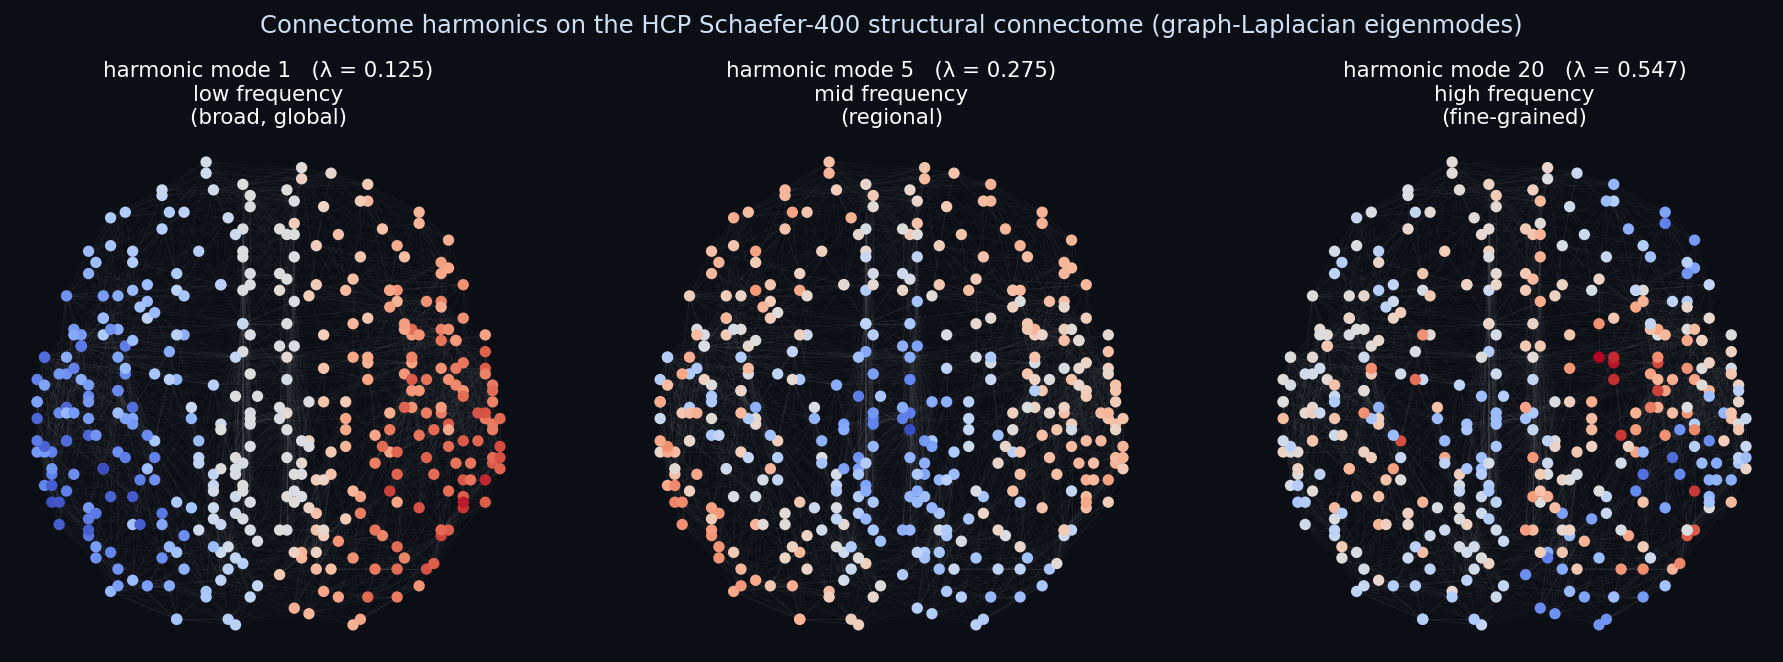
\includegraphics[width=\linewidth]{connectome_harmonic_modes.png}
  \caption{\textbf{Connectome harmonics on the brain.} Three graph-Laplacian
  eigenmodes of the HCP Schaefer-400 structural connectome, rendered on the
  cortical layout (red/blue = opposite sign of the standing-wave pattern; this is
  the basis the interactive demo animates). Low modes are broad and global, higher
  modes increasingly fine-grained; each mode's eigenvalue $\lambda$ gives its
  spatial frequency. Brain activity is reconstructed as weighted sums of such
  modes.}
  \label{fig:harmonics}
\end{figure}

A parallel line of work \cite{pang2023} has argued that the \emph{geometry}
of the cortical surface --- captured by the eigenmodes of the Laplace--Beltrami
operator (LBO) on the cortical mesh --- predicts functional activity at least as
well as connectivity-derived modes, prompting an ongoing debate about whether
shape or wiring is the more fundamental constraint \cite{mansour2024}.

Here we unify these threads in a single, fully reproducible, parcellated pipeline.
Working at the Schaefer-400 parcellation, we (i) measure the LSD-induced change in
the connectome-harmonic power spectrum, (ii) test whether the low-dimensional
harmonic embedding recovers known functional networks without supervision, and
(iii) directly compare connectome, geometric, and distance-based bases for their
ability to reconstruct the BOLD signal, asking whether the relative advantage of
geometry over wiring \emph{shifts} under a psychedelic. Crucially, we treat the
within-subject design as the source of statistical power: every subject provides
both drug and control states, so we test each subject's own drug-minus-control
difference. We then ask the strongest question available to us --- whether the
LSD effect \emph{replicates} in an independent psilocybin dataset acquired on a
different scanner with a different preprocessing pipeline and an active
(stimulant) placebo.

\section{Data and Methods}

\subsection{Datasets}
\textbf{Structural connectome.} A group-average HCP Young-Adult structural
connectivity matrix, parcellated to the Schaefer-400 atlas (400 cortical
regions, 7-network Yeo assignment), provides the weighted graph $W$.

\textbf{LSD fMRI (\texttt{ds003059}).} Resting-state fMRI from the Carhart-Harris
LSD study \cite{carharthtarris2020}, OpenNeuro \texttt{ds003059}, $n=12$
within-subject (each subject scanned under LSD and placebo). Volumetric data were
parcellated to Schaefer-400.

\textbf{Psilocybin fMRI (\texttt{ds006072}).} A precision-imaging psilocybin trial
\cite{siegel2025}, OpenNeuro \texttt{ds006072}, $n=7$ within-subject, comparing
psilocybin (25\,mg) against an \emph{active} placebo (methylphenidate, 40\,mg).
We used the provided fsLR-32k surface CIFTI dense time series (bandpassed, no
global-signal regression), parcellated to Schaefer-400 by averaging grayordinates
within each parcel. This is a methodologically cleaner, surface-based path than
the volumetric LSD pipeline, and an entirely independent cohort, scanner, and
preprocessing stream --- the key ingredients of a genuine replication.

\textbf{Cortical geometry.} Geometric eigenmodes were computed as LBO eigenmodes
of the fsLR-32k midthickness surface (NSBLab/BrainEigenmodes \cite{pang2023})
using LaPy, then parcellated to Schaefer-400.

\subsection{Bases}
We compare three orthonormal bases on the 400 parcels:
\begin{itemize}
  \item \textbf{Connectome harmonics}: eigenvectors of the symmetric normalized
  graph Laplacian
  \begin{equation}
    L = I - D^{-1/2}\,W\,D^{-1/2},
  \end{equation}
  where $D$ is the degree matrix of $W$. Eigenvalues order the harmonics by
  spatial frequency.
  \item \textbf{Geometric eigenmodes}: parcellated LBO eigenmodes of the cortical
  surface (shape, no wiring).
  \item \textbf{Exponential distance rule (EDR)}: eigenmodes of a surrogate
  connectome whose edge weights decay as $\exp(-d/\lambda)$ with inter-region
  distance $d$ and length constant $\lambda=20$\,mm --- geometry expressed as a
  network, with no real wiring.
\end{itemize}

\subsection{Reconstruction-accuracy comparison}
For each basis we reconstruct every parcellated BOLD frame from its first $N$
modes and score the reconstruction by its spatial correlation with the original,
averaged over frames, for $N$ on a logarithmic grid ($1\ldots200$). The area
under this accuracy-versus-$N$ curve (AUC) summarizes how efficiently a basis
recreates the data: a more natural basis reaches high accuracy with fewer modes.
For each subject and state we compute the \emph{basis advantage}
$\mathrm{AUC}(\text{geometric})-\mathrm{AUC}(\text{connectome})$.

\paragraph{Two distinct contrasts (and why EDR is not wiring).} It is essential
to keep two comparisons separate. The \emph{geometry-vs-wiring} contrast,
$\mathrm{AUC}(\text{geometric})-\mathrm{AUC}(\text{connectome})$, pits cortical
\emph{shape} against the \emph{real structural connectome} --- including its
long-range tracts --- and is the headline of this paper. The
\emph{geometry-vs-distance} contrast,
$\mathrm{AUC}(\text{geometric})-\mathrm{AUC}(\text{EDR})$, pits shape against a
\emph{distance-decay surrogate}; because EDR encodes only ``connections fall off
with distance'' it is itself a geometric object, \emph{not} a model of wiring.
A shift in the first contrast is a statement about shape versus wiring; a shift
in the second is a statement about two flavours of geometry and must not be read
as a wiring result.

\subsection{Harmonic consonance metric (Experiment 4)}
To probe the Symmetry Theory of Valence (STV)~\cite{johnson2016}, which posits
that the pleasantness of an experience tracks the \emph{symmetry} of its neural
representation and which has been operationalized on connectome harmonics via
musical-style \emph{consonance}, we summarize the harmonic power spectrum of each
subject and state. We project the (spatially centred, $z$-scored) parcellated BOLD
onto the orthonormal connectome harmonics, obtaining the time-averaged relative
power $p_k$ in mode $k$ ($\sum_k p_k=1$), and assign each mode the spatial
frequency $\omega_k=\sqrt{\lambda_k}$ from its Laplacian eigenvalue. From
$\{\omega_k,p_k\}$ we compute: (i) the \textbf{Sethares}~\cite{sethares1993}
\emph{sensory dissonance} of the spectrum treated as a chord, with $\omega_k$
mapped proportionally to an audio range (so frequency \emph{ratios}, hence
consonance relations, are preserved and identical across conditions; lower
dissonance $=$ more consonant); (ii) the normalized \textbf{spectral entropy} of
$p$ (repertoire breadth); and (iii) the \textbf{spectral centroid}
$\sum_k p_k\omega_k$ (energy toward high spatial frequency). Each metric is
submitted to the same within-subject paired test, exact sign-flip permutation
null, and GSR robustness rerun as the basis advantage. We also recompute all
metrics on the geometric harmonics as a substrate check.

\subsection{Statistics}
The within-subject \emph{shift} is the per-subject change in basis advantage
between drug and control (LSD$-$placebo, or psilocybin$-$methylphenidate). We
report the mean shift with its 95\% confidence interval, a paired $t$-test, the
nonparametric Wilcoxon signed-rank test, Cohen's $d_z$ effect size, and an
\emph{exact} within-subject sign-flip permutation test (all $2^n$ label
assignments: $4096$ for $n=12$, $128$ for $n=7$). At small $n$ the exact
permutation and Wilcoxon tests are the appropriate inferential tools; we note
that the smallest attainable two-sided permutation $p$-value is $2/2^n$
($\approx 0.0005$ at $n=12$, $\approx 0.016$ at $n=7$), so the psilocybin design
is intrinsically power-limited.

\subsection{Robustness / nuisance regression}
Because the raw LSD dataset lacks fmriprep motion parameters, we apply the
strongest nuisance model computable from the parcel time series alone:
linear$+$quadratic detrending, global-signal regression (GSR, plus its temporal
derivative), and DVARS-based Tukey-fence frame censoring. We then rerun the
identical paired and permutation tests on the denoised data. GSR removes the
dominant motion/arousal confound for drug-state contrasts, so survival of the
effect after GSR is our honest bottom line.

\subsection{Reproducibility}
All analyses are scripted in Python (\texttt{numpy}, \texttt{scipy},
\texttt{nibabel}, \texttt{nilearn}, \texttt{lapy}) with pinned dependency
versions. Data are fetched programmatically from their original sources. Code,
precomputed results, and an interactive browser demonstration are available at
\url{https://github.com/fractastical/connectome_harmonics} (live demo:
\url{https://fractastical.github.io/connectome_harmonics/}).

\section{Results}

\subsection{Experiment 1: LSD reorganizes the harmonic spectrum (in direction)}
Projecting ds003059 BOLD onto the HCP connectome harmonics, low-frequency
harmonics carry less power under LSD: the group mean low-band LSD/placebo power
ratio is $0.77$ and the high-band ratio is $0.85$ (Figure~\ref{fig:spectra}),
reproducing the \emph{direction} reported by Atasoy et al.\ \cite{atasoy2017}.
Repertoire entropy is essentially unchanged at this scale (LSD $3.614$ vs.\
placebo $3.607$). The high-frequency power \emph{increase} emphasized in the
original vertex-level work does not clearly separate at the coarse parcellated
resolution used here.

\begin{figure}[t]
  \centering
  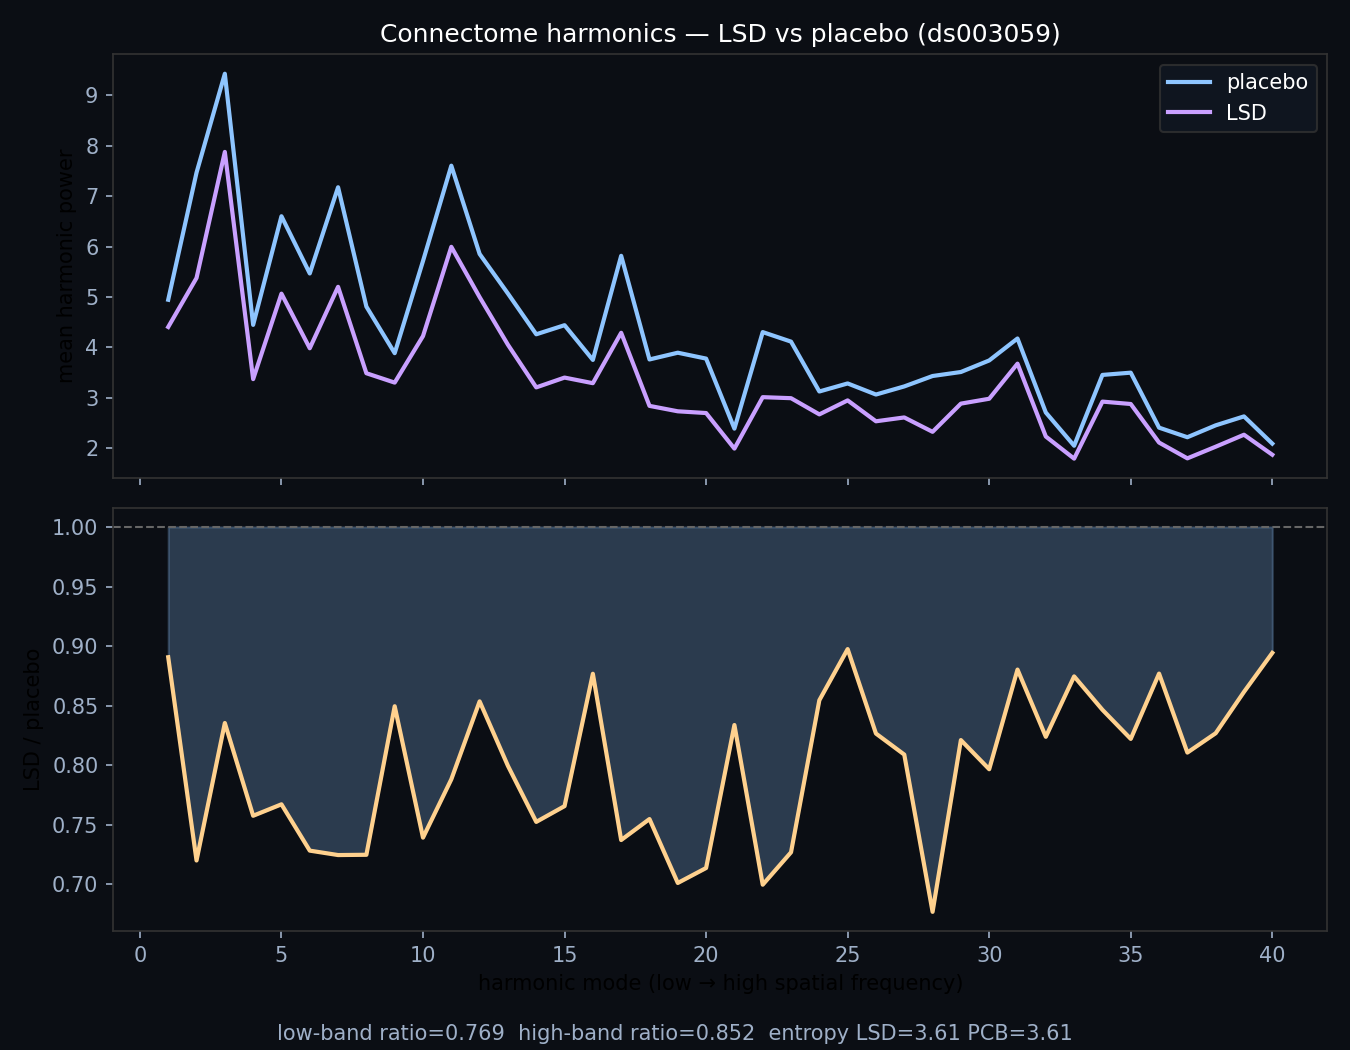
\includegraphics[width=0.85\linewidth]{lsd_harmonic_spectra.png}
  \caption{\textbf{Experiment 1.} Group-mean connectome-harmonic power versus
  spatial frequency (mode index), LSD versus placebo ($n=12$, ds003059), with the
  per-mode LSD/placebo power ratio below. Low-frequency modes are suppressed under
  LSD (low-band ratio $0.77$).}
  \label{fig:spectra}
\end{figure}

\subsection{Experiment 2: an unsupervised geometric latent space}
Using the lowest non-trivial harmonics as coordinate axes (a Laplacian
eigenmap), all 400 regions embed into a low-dimensional space in which the seven
Yeo functional networks separate into a continuous layout, ordered along the
first harmonic axis as Default-mode $\rightarrow$ Dorsal-attention
$\rightarrow$ Somatomotor $\rightarrow$ Salience/Ventral-attention $\rightarrow$
Limbic $\rightarrow$ Frontoparietal-control $\rightarrow$ Visual. No functional
labels were provided to the embedding: the organization emerges from structural
connectivity alone, consistent with the existence of a smooth functional gradient
encoded geometrically in the connectome.

\subsection{Experiment 3: shape versus wiring, and the LSD shift}
At 400-region resolution all three bases reconstruct the BOLD signal comparably
(Figure~\ref{fig:basis}, left/middle), with the distance-only EDR basis achieving
the best AUC in both states --- geometry does at least as well as wiring
(Table~\ref{tab:auc}). The novel result is the \emph{shift}: the per-subject
geometric$-$connectome advantage is negative under placebo ($-0.0021$) but
positive under LSD ($+0.0037$), a within-subject increase of
$\Delta\mathrm{AUC}=+0.0058$ (95\% CI $[+0.0030,+0.0085]$; paired $t(11)=4.60$,
$p=0.0008$; Wilcoxon $p=0.001$; exact permutation $p=0.001$; $d_z=1.33$, large),
with geometry gaining in all 12/12 subjects (Figure~\ref{fig:basis}, right).
After detrending, GSR, and DVARS censoring (98\% of frames retained) the effect
attenuates by roughly a quarter but remains significant
($\Delta\mathrm{AUC}=+0.0044$, paired $p=0.002$, permutation $p=0.003$,
$d_z=1.19$): it is not merely a motion or global-signal artifact.

\begin{table}[t]
  \centering
  \small
  \caption{Reconstruction AUC by basis and state. Higher is better.
  $\Delta_{\text{geo}-\text{conn}}$ is the geometric$-$connectome advantage.}
  \label{tab:auc}
  \begin{tabular}{llccc}
    \toprule
    Dataset & State & Connectome & Geometric & EDR \\
    \midrule
    LSD (ds003059, $n{=}12$) & Placebo & 0.7668 & 0.7647 & \textbf{0.7817} \\
                             & LSD     & 0.7515 & 0.7552 & \textbf{0.7730} \\
    \midrule
    Psilocybin (ds006072, $n{=}7$) & Methylphenidate & 0.7149 & 0.7051 & \textbf{0.7120} \\
                                   & Psilocybin      & 0.6914 & 0.6928 & \textbf{0.7002} \\
    \bottomrule
  \end{tabular}
\end{table}

\begin{figure}[t]
  \centering
  
\includegraphics[width=\linewidth]{basis_comparison.png}
  \caption{\textbf{Experiment 3 (LSD).} Reconstruction accuracy versus number of
  modes for each basis under placebo (left) and LSD (middle), and the per-subject
  paired shift of the geometric$-$connectome advantage (right). Nearly every
  subject moves toward geometry under LSD; the white/blue lines show the raw and
  nuisance-regressed group means.}
  \label{fig:basis}
\end{figure}

\subsection{Replication: the shift recurs under psilocybin}
We reran the identical paired analysis on the independent psilocybin cohort
(ds006072; psilocybin vs.\ active-placebo methylphenidate; $n=7$). The effect
replicates \emph{in direction} with a large effect size: the geometric$-$connectome
advantage shifts toward geometry by $\Delta\mathrm{AUC}=+0.0103$ (95\% CI
$[-0.0006,+0.0213]$; $d_z=0.87$). It is significant by the appropriate
nonparametric tests --- exact sign-flip permutation $p=0.031$ and Wilcoxon
$p=0.031$ --- and borderline by the parametric paired $t$-test
($t(6)=2.30$, $p=0.061$). Under aggressive GSR the effect attenuates to
$\Delta\mathrm{AUC}=+0.0061$ ($d_z=0.63$) and slips just below significance
(permutation $p=0.063$), mirroring the partial attenuation seen for LSD
(Figure~\ref{fig:psilo}, Table~\ref{tab:shift}). With $n=7$ against an active
stimulant placebo, the design is intrinsically underpowered; the converging
\emph{direction and effect size across two independent psychedelics} is the
substantive result, not any single $p$-value.

\begin{table}[t]
  \centering
  \small
  \caption{Within-subject shift in the geometric$-$connectome advantage
  (drug $-$ control). Permutation is the exact sign-flip test.}
  \label{tab:shift}
  \begin{tabular}{llccccc}
    \toprule
    Dataset & Data & $\Delta$AUC & paired $t$ ($p$) & Wilcoxon $p$ & perm.\ $p$ & $d_z$ \\
    \midrule
    LSD ($n{=}12$)        & Raw       & $+0.0058$ & $4.60$ ($0.0008$) & $0.001$ & $0.001$ & $1.33$ \\
                          & Denoised  & $+0.0044$ & $3.5$\;\;($0.002$) & $0.002$ & $0.003$ & $1.19$ \\
    \midrule
    Psilocybin ($n{=}7$)  & Raw       & $+0.0103$ & $2.30$ ($0.061$) & $0.031$ & $0.031$ & $0.87$ \\
                          & Denoised  & $+0.0061$ & $1.68$ ($0.145$) & $0.078$ & $0.063$ & $0.63$ \\
    \bottomrule
  \end{tabular}
\end{table}

\begin{figure}[t]
  \centering
  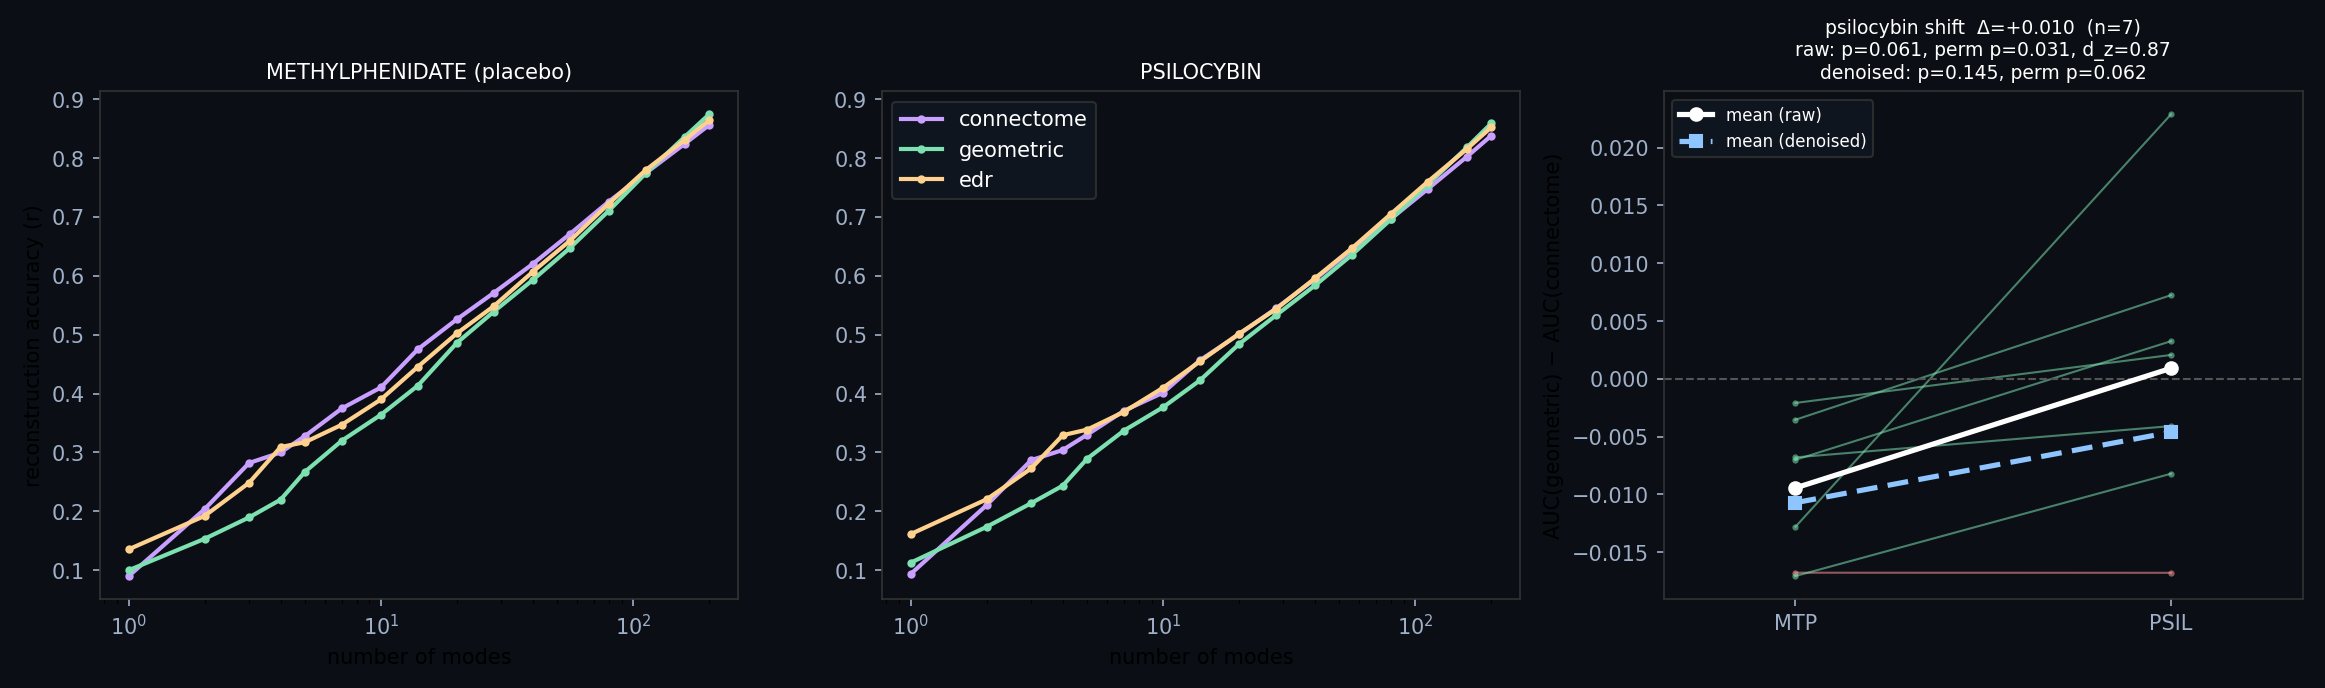
\includegraphics[width=\linewidth]{psilocybin_replication.png}
  \caption{\textbf{Replication (psilocybin, ds006072, $n=7$).} Same per-subject
  paired test on an independent drug, scanner, and pipeline: reconstruction
  accuracy under methylphenidate (left) and psilocybin (middle), and the
  per-subject shift (right). Activity again moves toward geometry under
  psilocybin ($\Delta\mathrm{AUC}=+0.010$, $d_z=0.87$, exact-permutation
  $p=0.031$).}
  \label{fig:psilo}
\end{figure}

\subsection{Vertex-resolution robustness check}
The principal limitation of the analyses above is their 400-region parcellation,
the regime in which the geometric advantage is weakest. We therefore repeated the
reconstruction comparison on the psilocybin cohort at \emph{vertex} resolution, in
fsaverage5 space (10{,}242 vertices, left hemisphere), the resolution at which Pang
et al.\ \cite{pang2023} publish eigenbases. The fsLR-32k BOLD was resampled to
fsaverage5 with a pure-Python area-average resampler built from registration-fusion
spheres (validated against native Laplace--Beltrami modes, $|r|=0.86$--$0.97$ for
the lowest modes). Two findings emerge (Figure~\ref{fig:vertex}).

First, the \textbf{geometric basis reconstructs vertex BOLD efficiently}
(AUC $\approx 0.32$--$0.34$), close to EDR ($\approx 0.30$--$0.32$): the geometry
result is not an artifact of parcellation.

Second, and reported in the interest of full honesty, a fair geometry-versus-\emph{wiring}
test is \textbf{not possible at vertex resolution with public data}. The only
publicly available connectome modes are a synthetic demo surrogate (degenerate
spectrum, near-zero reconstruction), and real tractography connectome eigenmodes are
not released at vertex resolution. The geometry-vs-wiring shift therefore remains a
parcellated result. The contrast we \emph{can} evaluate at vertex resolution,
geometry vs.\ EDR (shape vs.\ distance), shows a small but significant shift of the
\emph{opposite} sign to the parcellated geometry-vs-connectome shift:
$\Delta(\text{geometric}-\text{EDR})=-0.0067$, 95\% CI $[-0.011,-0.002]$,
paired $t(6)=-3.55$ ($p=0.012$), Wilcoxon/permutation $p=0.031$, $d_z=-1.34$. The
``toward geometry'' effect is thus \emph{specific to the geometry-vs-wiring contrast}
and does not generalize to geometry-vs-distance at fine scale; overall reconstruction
also drops modestly under psilocybin for both bases. The parcellated headline is
about cortical shape versus \emph{specific wiring}, not a blanket claim that geometry
wins under psychedelics at every scale and contrast.

\begin{figure}[t]
  \centering
  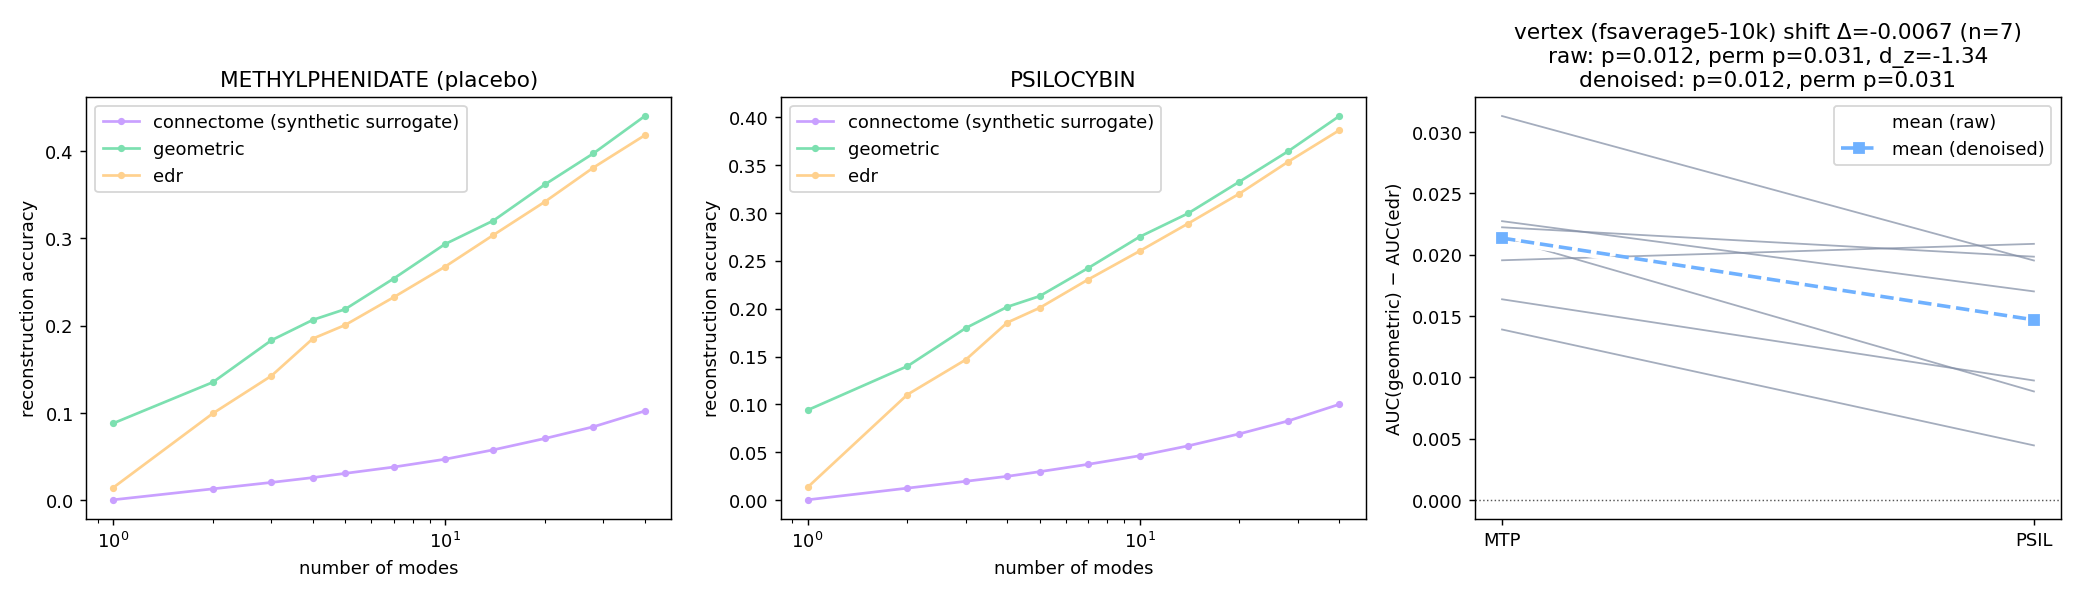
\includegraphics[width=\linewidth]{vertex_basis_comparison.png}
  \caption{\textbf{Vertex-resolution check (psilocybin, fsaverage5-10k, $n=7$, left
  hemisphere).} Reconstruction accuracy under methylphenidate (left) and psilocybin
  (middle) for the geometric and EDR bases (the public connectome basis is a synthetic
  surrogate that reconstructs near zero and is shown only for reference). Right:
  per-subject geometric$-$EDR advantage, which shifts slightly toward EDR under
  psilocybin ($\Delta=-0.0067$, permutation $p=0.031$).}
  \label{fig:vertex}
\end{figure}

\subsection{Experiment 4: harmonic consonance decreases under psychedelics}
A natural extension asks whether the degree of geometric/harmonic order relates to
affect, as the Symmetry Theory of Valence~\cite{johnson2016} proposes. We cannot
test this correlation directly --- neither public release ships per-subject affect
ratings --- so we test the prerequisite \emph{mechanism direction}: does a
serotonergic psychedelic move the harmonic spectrum toward consonance/symmetry, or
away from it? The answer is unambiguous and runs \emph{against} the naive STV
prediction (Figure~\ref{fig:consonance}). Under LSD the connectome-harmonic
spectrum becomes markedly \textbf{more dissonant} (drug$-$placebo
$\Delta=+16.7$, paired $p=0.001$, exact permutation $p=0.002$, $d_z=1.24$),
\textbf{broader} (spectral entropy $p=0.007$), and shifted toward \textbf{higher}
spatial frequencies (centroid $p=0.015$); all three survive global-signal
regression and frame censoring. Psilocybin ($n=7$) trends in the same direction on
every metric but does not reach significance (dissonance $\Delta=+11.0$, $d_z=0.49$,
$p=0.24$). On the geometric-harmonic substrate the LSD dissonance increase is
weaker but same-signed ($\Delta=+2.1$, $p=0.022$).

This is the ``entropic brain'' direction~\cite{atasoy2017} and clarifies a subtle
point: the drift toward the smooth geometric \emph{basis} in Experiment 3 is
\emph{not} the same as increased \emph{consonance}. Activity can gain on the wiring
basis relative to shape while the overall power spectrum simultaneously spreads to
higher, less harmonically related modes. If anything, a simple spatial-consonance
reading of STV predicts the wrong sign for the (typically positively-valenced)
acute psychedelic state; we discuss the caveats to that inference below.

\begin{figure}[t]
  \centering
  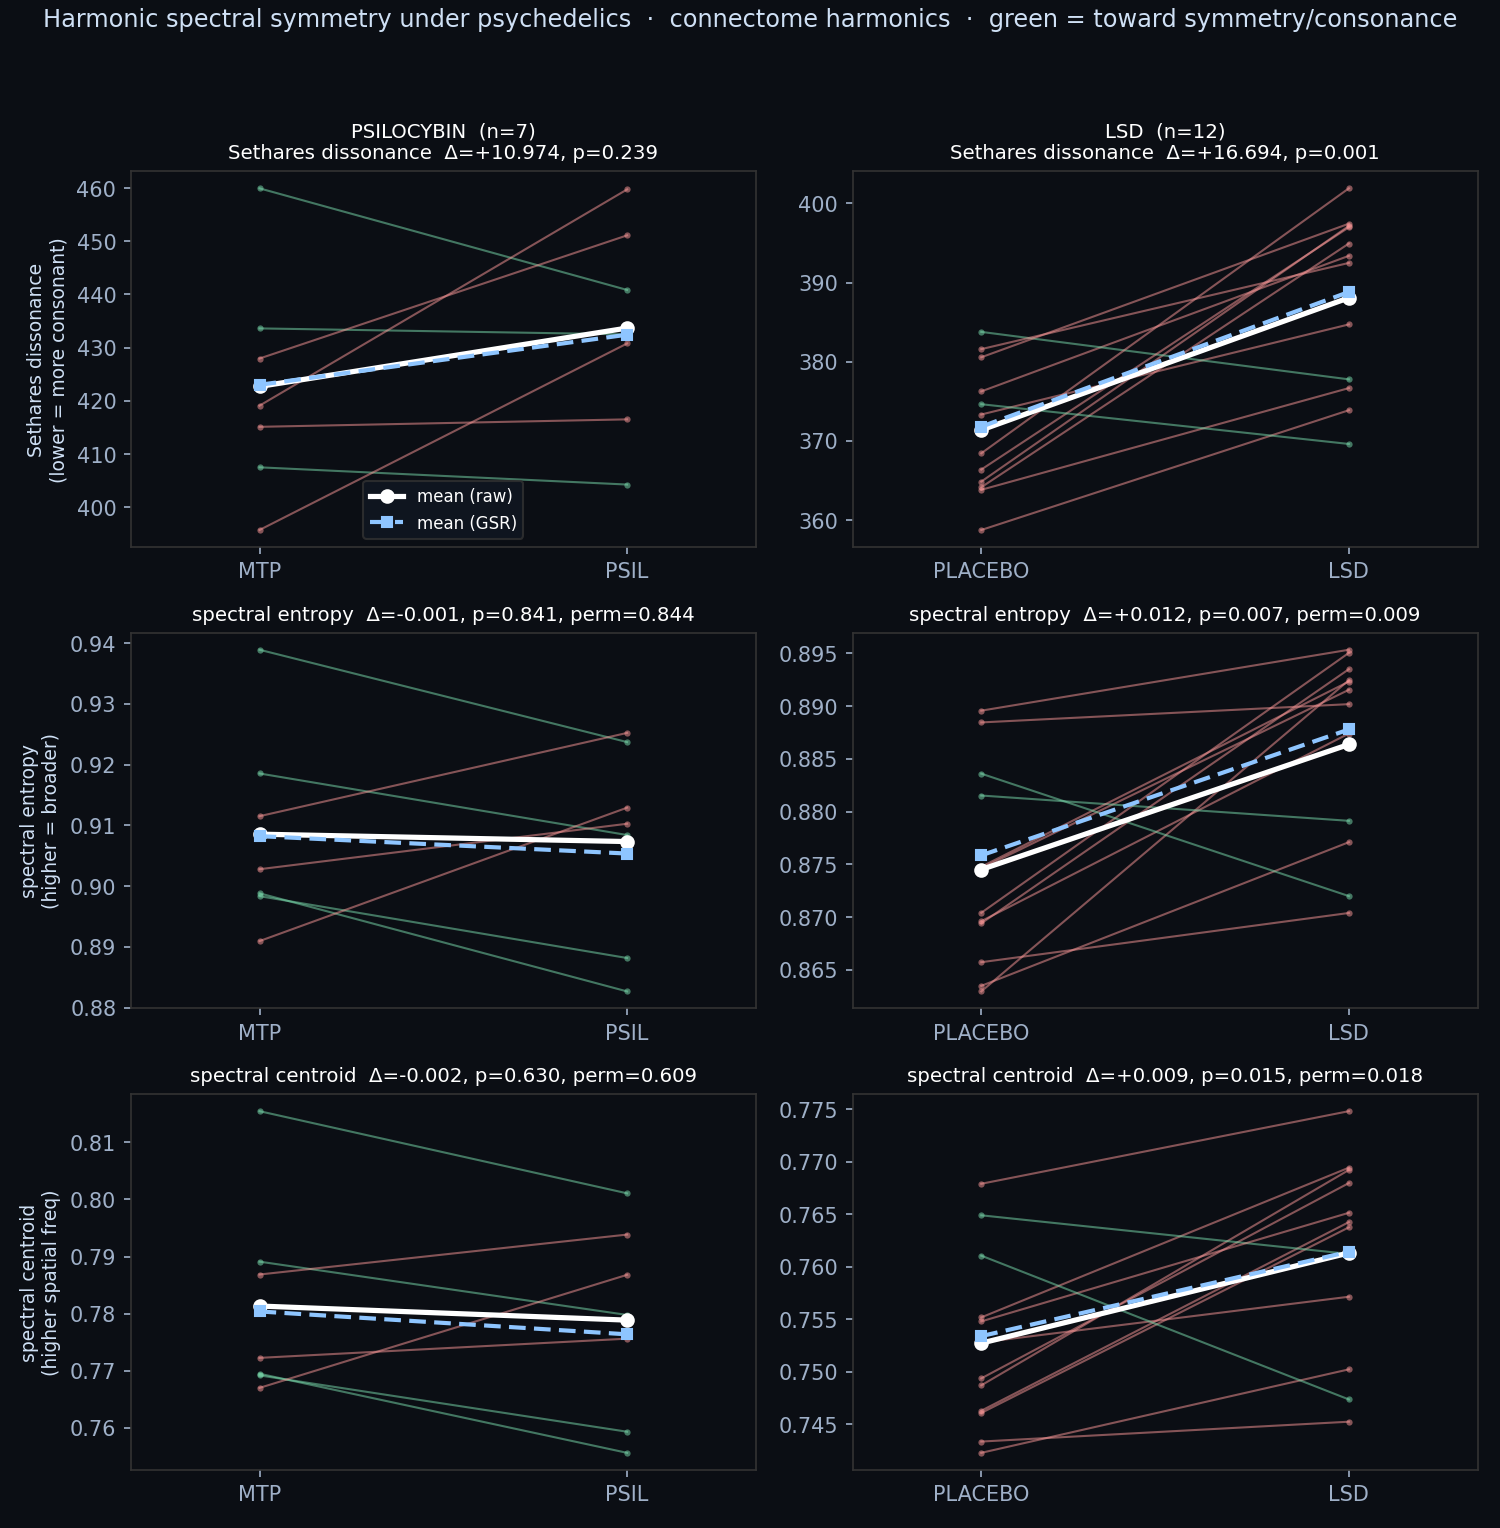
\includegraphics[width=\linewidth]{harmonic_consonance.png}
  \caption{\textbf{Harmonic consonance / spectral symmetry under psychedelics
  (connectome harmonics).} Per-subject paired change (placebo$\to$drug) in Sethares
  dissonance (top), spectral entropy (middle), and spectral centroid (bottom), for
  psilocybin (left, $n=7$) and LSD (right, $n=12$); green lines move toward
  symmetry/consonance, red away. White $=$ raw means, blue dashed $=$ after GSR.
  Under LSD nearly every subject moves away from consonance (more dissonant,
  broader, higher-frequency); psilocybin trends the same way.}
  \label{fig:consonance}
\end{figure}

\section{Discussion}
Across two independent psychedelic datasets, cortical activity shifts toward a
smoother, shape-aligned (geometric) description and away from one tied to specific
structural wiring. The LSD effect is strong and survives our nuisance model; the
psilocybin effect, in a smaller and harder (active-placebo) design, replicates the
direction and effect size and is significant by exact nonparametric tests on raw
data. Together with the spectral reorganization of Experiment 1 (less
low-frequency, wiring-bound structure under LSD) and the unsupervised geometric
latent space of Experiment 2, the picture is coherent: psychedelics appear to
relax activity off the connectome's specific scaffolding toward the broad
geometric modes that the cortex's shape most readily supports.

\paragraph{Consonance and valence.} Experiment 4 adds an important qualification.
The same psychedelic state that aligns activity with smooth geometric modes also
makes the harmonic power spectrum \emph{less} consonant and broader --- the
opposite of what a literal spatial-consonance reading of the Symmetry Theory of
Valence~\cite{johnson2016} would predict for a typically positive state. We stress
that this is not a refutation of STV: we measure \emph{spatial}-harmonic, not
temporal, consonance; the acute psychedelic state is variably (not uniformly)
valenced; and the ``neural annealing'' formulation of STV explicitly predicts a
transient rise in energy and entropy (``heating'') before any annealing toward
order, so a snapshot of increased breadth during the drug condition is consistent
with that account. Most importantly, without per-subject affect ratings --- absent
from both public datasets --- we test only the mechanism direction, not the
valence correlation itself. The result is best read as a sharp, falsifiable
prediction generator: it shows that ``more geometric alignment'' and ``more
harmonic consonance'' are dissociable, and that a proper STV test will require
datasets pairing connectome-harmonic decompositions with validated affect scales.

\paragraph{Limitations.} All results are group-average and/or parcellated at 400
regions --- precisely the regime in which the geometric advantage over wiring is
weakest, and in which geometric modes are hemisphere-separable while connectome
and EDR modes are whole-brain. We therefore frame Experiment 3 as a test of the
drug-induced \emph{shift}, not as a resolution of the broader geometry-versus-wiring
debate, which requires vertex-resolution surfaces and carefully constructed
connectomes \cite{mansour2024}; our own vertex-resolution attempt
(Section~3.5) confirms that a fair geometry-vs-wiring comparison is currently
blocked by the absence of public real-connectome eigenmodes at that resolution.
The LSD data lack fmriprep motion parameters, so
no full 24-parameter motion regression is possible; after denoising neither basis
significantly beats the other within a single state (the claim is about the shift).
Sample sizes are modest ($n=12$ and $n=7$), and the psilocybin cohort uses an
active stimulant placebo, which makes its design conservative but underpowered.
These are reanalyses of public data and are not clinical or individual-level
findings, and not medical advice.

\paragraph{Conclusion.} A simple, reproducible, parcellated pipeline shows that
the relative fit of cortical \emph{shape} versus \emph{wiring} to brain activity
is state-dependent and bends toward geometry under both LSD and psilocybin. We
release all code, fetch scripts, precomputed results, and an interactive demo to
support scrutiny and extension to vertex-resolution data.

\section*{Data and Code Availability}
Code, analysis scripts, precomputed results, and an interactive web demonstration:
\url{https://github.com/fractastical/connectome_harmonics}. Primary data are public:
HCP-YA structural connectivity (Human Connectome Project terms apply), OpenNeuro
\texttt{ds003059} (LSD), and OpenNeuro \texttt{ds006072} (psilocybin). Cortical
surfaces, parcellations, and eigenmode tooling from NSBLab/BrainEigenmodes and
ThomasYeoLab/CBIG retain their own licenses.

\section*{Acknowledgments}
This work was sponsored by the California Institute of Machine Consciousness. We
thank the OpenNeuro contributors and the authors of the original LSD and
psilocybin studies for making their data public.

\begin{thebibliography}{9}
\bibitem{atasoy2016} Atasoy, S., Donnelly, I., \& Pearson, J. (2016).
Human brain networks function in connectome-specific harmonic waves.
\emph{Nature Communications}, 7, 10340.

\bibitem{atasoy2017} Atasoy, S., Roseman, L., Kaelen, M., Kringelbach, M. L.,
Deco, G., \& Carhart-Harris, R. L. (2017). Connectome-harmonic decomposition of
human brain activity reveals dynamical repertoire re-organization under LSD.
\emph{Scientific Reports}, 7, 17661.

\bibitem{carharthtarris2020} Carhart-Harris, R. L., et al. (2016/2020).
LSD resting-state fMRI dataset. OpenNeuro \texttt{ds003059}.
\url{https://openneuro.org/datasets/ds003059}.

\bibitem{pang2023} Pang, J. C., Aquino, K. M., Oldehinkel, M., et al. (2023).
Geometric constraints on human brain function. \emph{Nature}, 618, 566--574.

\bibitem{mansour2024} Mansour L., S., Tian, Y., Fornito, A., et al. (2024).
The relative contributions of connectome geometry and wiring to brain function
(preprint). \emph{bioRxiv} 2024.04.16.589843.

\bibitem{siegel2025} Siegel, J. S., et al. (2025). Psilocybin precision
functional imaging dataset. \emph{Scientific Data}.
OpenNeuro \texttt{ds006072}. \url{https://openneuro.org/datasets/ds006072}.

\bibitem{johnson2016} Johnson, M. E. (2016). \emph{Principia Qualia: Blueprint
for a New Science}. Qualia Research Institute.
\url{https://opentheory.net/PrincipiaQualia/}.

\bibitem{sethares1993} Sethares, W. A. (1993). Local consonance and the
relationship between timbre and scale. \emph{Journal of the Acoustical Society of
America}, 94(3), 1218--1228.
\end{thebibliography}

\end{document}
